\documentclass[a4paper,oneside,12pt]{extreport}

\usepackage{mmap}
\usepackage[T2A]{fontenc}
\usepackage[utf8]{inputenc}
\usepackage[english,russian]{babel}


% Текст отчёта следует печатать, соблюдая следующие размеры полей:
% левое — 30 мм, правое — 15 мм, верхнее и нижнее — 20 мм.
\usepackage[left=20mm, right=15mm, top=15mm, bottom=15mm]{geometry}

% \setlength{\parindent}{1.25cm} % Абзацный отступ

\usepackage{setspace}
%\onehalfspacing % Полуторный интервал

\frenchspacing % Равномерные пробелы
\usepackage{indentfirst} % Красная строка

\usepackage{microtype}
\sloppy

\usepackage{titlesec}
\titlespacing*{\chapter}{0pt}{-30pt}{8pt}
\titlespacing*{\section}{\parindent}{*4}{*4}
\titlespacing*{\subsection}{\parindent}{*4}{*4}
\titleformat{\chapter}{\LARGE\bfseries}{\thechapter}{20pt}{\LARGE\bfseries}
\titleformat{\section}{\Large\bfseries}{\thesection}{40pt}{\Large\bfseries}

\usepackage{graphicx}
\usepackage{caption}

\usepackage[unicode,pdftex]{hyperref}
\hypersetup{hidelinks}

%% title begin
\usepackage{wrapfig}

\makeatletter
	\def\vhrulefill#1{\leavevmode\leaders\hrule\@height#1\hfill \kern\z@}
\makeatother
%% title end

%% begin code
\usepackage{listings}
\usepackage{xcolor}

\lstset{
	basicstyle=\footnotesize\ttfamily,
	breakatwhitespace=true,
	breaklines=true,
	commentstyle=\color{gray},
	frame=single,
	keywordstyle=\color{blue},
	stringstyle=\color{red},
	tabsize=8
}

\lstdefinestyle{lispinline}{
	frame=none,
	language=Lisp
}

\newcommand{\code}[1]{\texttt{#1}}
%% end code

%% begin theorem
\usepackage{amsthm}

\makeatletter
\newtheoremstyle{indented}
	{}% measure of space to leave above the theorem
	{}% measure of space to leave below the theorem
	{}% name of font to use in the body of the theorem
	{\parindent}% measure of space to indent
	{\bfseries}% name of head font
	{.}% punctuation between head and body
	{ }% space after theorem head; " " = normal interword space
	{}% header specification (empty for default)
\makeatother

\theoremstyle{indented}

\newtheorem{definition}{Определение}[section]
\newtheorem{example}{Пример}[section]
\newtheorem{theorem}{Теорема}[section]
\newtheorem{task}{Задание}

\makeatletter
\DeclareRobustCommand\bfseriesitshape{%
	\not@math@alphabet\itshapebfseries\relax
	\fontseries\bfdefault
	\fontshape\itdefault
	\selectfont
}
\makeatother

\DeclareTextFontCommand{\textbfit}{\bfseriesitshape}
\DeclareTextFontCommand{\define}{\bfseriesitshape}
%% end theorem

%% begin columns
\usepackage{etoolbox,refcount}
\usepackage{multicol}

\newcounter{countitems}
\newcounter{nextitemizecount}
\newcommand{\setupcountitems}{%
	\stepcounter{nextitemizecount}%
	\setcounter{countitems}{0}%
	\preto\item{\stepcounter{countitems}}%
}
\makeatletter
\newcommand{\computecountitems}{%
	\edef\@currentlabel{\number\c@countitems}%
	\label{countitems@\number\numexpr\value{nextitemizecount}-1\relax}%
}
\newcommand{\nextitemizecount}{%
	\getrefnumber{countitems@\number\c@nextitemizecount}%
}
\newcommand{\previtemizecount}{%
	\getrefnumber{countitems@\number\numexpr\value{nextitemizecount}-1\relax}%
}
\makeatother
\newenvironment{AutoMultiColItemize}{%
	\ifnumcomp{\nextitemizecount}{>}{3}{\begin{multicols}{2}}{}%
		\setupcountitems\begin{itemize}}%
		{\end{itemize}%
		\unskip\computecountitems\ifnumcomp{\previtemizecount}{>}{3}{\end{multicols}}{}}
\makeatother
\newenvironment{AutoMultiColEnumerate}{%
	\ifnumcomp{\nextitemizecount}{>}{3}{\begin{multicols}{2}}{}%
		\setupcountitems\begin{enumerate}}%
		{\end{enumerate}%
		\unskip\computecountitems\ifnumcomp{\previtemizecount}{>}{3}{\end{multicols}}{}}
%% end columns



\begin{document}

\begin{titlepage}
	{\large % 14pt instead of 12pt
	\onehalfspacing
	\centering

	\begin{wrapfigure}[7]{l}{0.14\linewidth}
		\vspace{3mm}
		\hspace{-10mm}
		
\includegraphics[width=\linewidth]{img/b_logo}
		% \includegraphics[width=0.93\linewidth]{inc/img/bmstu-logo}
	\end{wrapfigure}
	{\singlespacing \footnotesize \bfseries Министерство науки и высшего образования Российской Федерации\\Федеральное государственное бюджетное образовательное учреждение\\высшего образования\\<<Московский государственный технический университет\\имени Н.~Э.~Баумана\\ (национальный исследовательский университет)>>\\(МГТУ им. Н.~Э.~Баумана)\\}

	\vspace{-2.2mm}
	\vhrulefill{0.9mm}\\
	\vspace{-7.5mm}
	\vhrulefill{0.2mm}\\
	\vspace{2mm}

	{\doublespacing \small \raggedright ФАКУЛЬТЕТ \hspace{5mm} \underline{«Информатика и системы управления»}\\
	КАФЕДРА \hspace{10mm} \underline{«Программное обеспечение ЭВМ и информационные технологии»}\\}

	\vspace{20mm}

	\begin{center}
		\noindent\begin{minipage}{1.2\textwidth}\centering
			\textbf{ОТЧЕТ ПО ЛАБОРАТОРНОЙ РАБОТЕ №18,19}\newline
			\textbf{По курсу: "Функциональное и Логическое программирование"}\newline\newline\newline
		\end{minipage}
	\end{center}

	\vspace{20mm}

	\noindent ~~Тема \underline{~~~~~~~~~~~~~~~~~~~~~~~~~~Рекурсия в прологе.~~~~~~~~~~~~~~~~~~~~~~~~~~~~~~~~~~~~~~~~~~~}\newline
	\noindent ~~Группа \underline{~~~~~~~~~~~~~~~~~~~~~~~~~~~~~~~~~~~ИУ7-63Б~~~~~~~~~~~~~~~~~~~~~~~~~~~~~~~~~~~~~~~~~~~~~~~~~}\newline
	\noindent ~~Студент \underline{~~~~~~~~~~~~~~~~~~~~~~~~~~~~Сукочева А.~~~~~~~~~~~~~~~~~~~~~~~~~~~~~~~~~~~~~~~~~~~~~~~~~~}\newline
	\noindent ~~Преподаватель \underline{~~~~~~~~~~~~~~~~~Толпинская Н.Б.~~~~~~~~~~~~~~~~~~~~~~~~~~~~~~~~~~~~~~~~~~~~~}\newline
	\noindent ~~Преподаватель \underline{~~~~~~~~~~~~~~~~~~Строганов Ю. В.~~~~~~~~~~~~~~~~~~~~~~~~~~~~~~~~~~~~~~~~~~~~}\newline


	\begin{center}
		\vfill
		Москва~---~\the\year
		~г.
	\end{center}
	}



\end{titlepage}

\setcounter{page}{2}

\section*{Практическая часть}

\begin{task}
    Написать функцию, которая по своему списку-аргументу \code{lst} определяет, является ли он палиндромом (то есть равны ли \code{lst} и \code{(reverse lst)}).

    \begin{lstlisting}[language=Lisp]
(defun same-rec (lst1 lst2)
(cond ((null lst1)) 
    ((= (car lst1) (car lst2)) (same-rec (cdr lst1) (cdr lst2)))
    (T Nil)) )

(defun same (lst1 lst2)
        (if (= (length lst1) (length lst2) ) 
            (same-rec lst1 lst2)) )

(defun is-palindrome (lst) 
    (same lst (reverse lst)))
    \end{lstlisting}

    Пример использования:
    \begin{lstlisting}[language=Lisp]    
(is-palindrome '(1 2 3 3 2 1))  ;; T
(is-palindrome '(1 2 3 2 1))    ;; T
(is-palindrome '(1 2 3 4))      ;; Nil
    \end{lstlisting}
\end{task}
		
\begin{task}
	Написать предикат \code{set-equal}, который возвращает \code{t}, если два его
    множества-аргумента содержат одни и те же элементы, порядок которых не имеет значения.


    \begin{lstlisting}[language=Lisp]
(defun find-elem-in-set (set1 elem) 
    (cond ((null set1) Nil)
        ((= (car set1) elem) T)
        (T (find-elem-in-set (cdr set1) elem)) ) )

(defun set-equal-rec (set1 set2) 
    (cond ((null set1))
        ((find-elem-in-set set2 (car set1)) (set-equal-rec (cdr set1) set2))
        (T Nil)) )

(defun set-equal (set1 set2)
    (if (= (length set1) (length set2)) 
        (set-equal-rec set1 set2) Nil) )
\end{lstlisting}

    Пример использования:
    \begin{lstlisting}[language=Lisp]
(set-equal '(1 2 3) '(4 5 6)) ;; Nil
(set-equal '(1 2 3) '(3 1 2)) ;; T
    \end{lstlisting}

\end{task}

\begin{task}
    Напишите необходимые функции, которые обрабатывают таблицу из точечных пар:
    
    (страна.столица), и возвращает по стране - столицу, а по столице - страну.
    \begin{lstlisting}[language=Lisp]
(defun find-capital (table country)
    (cond ((null table) Nil)
        ((eq (caar table) country) (cdar table)) 
        (T (find-capital (cdr table) country))) )

(defun find-country (table capital)
    (cond ((null table) Nil)
        ((eq (cdar table) capital) (caar table)) 
        (T (find-country (cdr table) capital))) )
    \end{lstlisting}

    Пример использования:
    \begin{lstlisting}[language=Lisp]
(find-capital 
    '((Russia . Moscow)
    (Spain . Madrid)
    (France . Paris)) 'Russia) ;; MOSCOW

(find-capital 
    '((Russia . Moscow)
    (Spain . Madrid)
    (France . Paris)) 'Hungary) ;; Nil


(find-country
    '((Russia . Moscow)
    (Spain . Madrid)
    (France . Paris)) 'Moscow) ;; RUSSIA

(find-country
    '((Russia . Moscow)
    (Spain . Madrid)
    (France . Paris)) 'Budapest) ;; Nil
    \end{lstlisting}

\end{task}

\begin{task}
	Напишите функцию \code{swap-first-last}, которая
    переставляет в списке-аргументе первый и последний элементы.
    
    Функция f1 возвращает все, кроме последнего
    \begin{lstlisting}[language=Lisp]
(defun f1 (lst)
    (reverse (cdr (reverse lst))) )
    \end{lstlisting}
    
    Функция swap-first-last добавляет к последнему элементу весь список 
    без последнего элемента, а к нему первый элемент.
    \begin{lstlisting}[language=Lisp]
(defun swap-first-last (lst)
    (append (append (last lst) (cdr (f1 lst))) (cons (car lst) Nil)))
    \end{lstlisting}

    Пример использования:
    \begin{lstlisting}[language=Lisp]
(swap-first-last '(1 2 3 4 5)) ;; (5 2 3 4 1)
(swap-first-last '(1 2)) ;; (2 1)
    \end{lstlisting}

\end{task}

\begin{task}
	Напишите функцию \code{swap-two-elements}, которая переставляет в списке-аргументе
    два указанных своими порядковыми номерами элемента в этом списке.

    \begin{lstlisting}[language=Lisp]
(defun my-length-rec (lst n)
    (cond 
    ((null lst) n)
    (T (my-length-rec (cdr lst) (+ n 1)))) )	

(defun my-length (lst)	
    (my-length-rec lst 0) )
    \end{lstlisting}

    Возвращает элемент по индексу.
    \begin{lstlisting}[language=Lisp]
(defun find-by-index-rec (lst index curr-index) 
    (cond ((null lst) Nil)
    ((= index curr-index ) (car lst))
    (T (find-by-index-rec (cdr lst) index (+ curr-index 1)))) )

(defun find-by-index (lst index) 
    (find-by-index-rec lst index 0))
    \end{lstlisting}

    \begin{lstlisting}[language=Lisp]
(defun swap-two-elements-rec (lst index1 index2 curr-index source-list)
    (cond ((null lst) nil)
        ((= curr-index index1) (cons (find-by-index source-list index2) (swap-two-elements-rec (cdr lst) index1 index2 (+ curr-index 1) source-list)))
        ((= curr-index index2) (cons (find-by-index source-list index1) (swap-two-elements-rec (cdr lst) index1 index2 (+ curr-index 1) source-list)))
        (T (cons (car lst) (swap-two-elements-rec (cdr lst) index1 index2 (+ curr-index 1) source-list) )) ) )
    \end{lstlisting}

    \begin{lstlisting}[language=Lisp]
(defun swap-two-elements (lst i1 i2)
    (cond 
    ((>= i1 (my-length lst)) 
    "The first index is larger than the size of the list")
    ((>= i2 (my-length lst)) 
    "The second index is larger than the size of the list")
    ((< i1 0) 
    "The first index is less than zero")
    ((< i2 0) 
    "The second index is less than zero")
    ((= i1 i2) lst)
    (T (swap-two-elements-rec lst i1 i2 0 lst))) )    
    \end{lstlisting}

    Пример использования:
    \begin{lstlisting}[language=Lisp]
(swap-two-elements '(11 12 13 14 15) 0 4) ;; (15 12 13 14 11)
(swap-two-elements '(11 12 13 14 15) 4 0) ;; (15 12 13 14 11)
(swap-two-elements '(11 12 13 14 15) 0 0) ;; (11 12 13 14 15)
    \end{lstlisting}

\end{task}

\begin{task}
    Напишите две функции, \code{swap-to-left} и \code{swap-to-right}, 
    которые производят круговую перестановку в списке-аргументе влево и вправо, соответственно.
    
    Возвращает список без последнего элемента.
    \begin{lstlisting}[language=Lisp]
(defun f1 (lst)
    (reverse (cdr (reverse lst))) )
    \end{lstlisting}

    \begin{lstlisting}[language=Lisp]
(defun f-last (lst)
        (car (reverse lst)) )
    \end{lstlisting}

    \begin{lstlisting}[language=Lisp]
(defun swap-to-right (lst)
    (cons (f-last lst) (f1 lst)))

(defun swap-to-left (lst)
	(append (cdr lst) (cons (car lst) nil)) )
    \end{lstlisting}

    Пример использования:
    \begin{lstlisting}[language=Lisp]
(swap-to-right '(1 2 3 4 5 6)) ;; (6 1 2 3 4 5)
(swap-to-left '(1 2 3 4 5 6))  ;;(2 3 4 5 6 1)
    \end{lstlisting}

\end{task}
      
      

    
% \begin{figure}[ht!]
% 	\centering{
% 		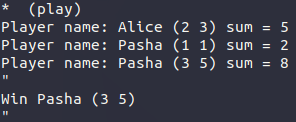
\includegraphics[width=0.5\textwidth]{img/5.png}
% 		\caption{Результат работы 5.} }
% \end{figure}

\newpage

\section*{Теоретическая часть}

\subsection*{Способы определения функции}


1. С помощью \code{lambda}. 

Базовое определение лямбда-выражения:

(lambda лямбда-список тело\_функции)

Пример:

\begin{lstlisting}[language=Lisp]
(lambda (x y) (+ x y))
\end{lstlisting}

Применение лямбда-выражений:

(лямбда-выражение фактические\_параметры)

Пример:

\begin{lstlisting}[language=Lisp]
((lambda (x y) (+ x y)) 1 2) ;; 3
\end{lstlisting}


2. С помощью \code{defun}. 
Для неоднократного применения функции (а также для построения
рекурсивной функции) используется встроенная функция defun.

Синтаксис:

(defun имя\_функции лямбда-список тело\_функции)

Пример:

\begin{lstlisting}[language=Lisp]
(defun sum (x y) (+ x y))
\end{lstlisting}

Пример вызова:

\begin{lstlisting}[language=Lisp]
(sum 1 2) ;; 3
\end{lstlisting}


\subsection*{Варианты и методы модификации элементов списков}

Функции для работы со списками делятся на две группы:

\begin{enumerate}
    \item Не разрушающие структуру. Если сохраняется возможность работать с исходными списками, значит функции не разрушают структуру.
    (Пример: append, reverse, length, subst ...)
    \item Разрушающие структуру. 
    Если после использования какой-то стандартной функции после ее работы теряется 
    возможность работы с теми списками, которые изначально были, значит их структура разрушилась. 
    Чаще всего такие функции начинаются в буквы 'n (Пример: nconc, nreverse, nsubst ...)
\end{enumerate}


\end{document}